\documentclass[10pt,a4paper]{article}
\usepackage[utf8]{inputenc}
\usepackage{fontenc}
\usepackage[french]{babel}
\usepackage[top=0.5cm, bottom=0.5cm, left=0.5cm, right=0.5cm]{geometry}
\usepackage{graphicx}
\usepackage{lmodern}
\usepackage{amsmath}
\usepackage{amssymb}
\usepackage{mathrsfs}
\usepackage{multirow}
\usepackage{schemabloc}
\usepackage[european resistors]{circuitikz}
\usepackage{array}
\usepackage{multicol}
%\usepackage{auto-pst-pdf}
%\usepackage[usenames,dvipsnames]{pstricks}
%\usepackage{pstricks}
%\usepackage{epsfig}
%\usepackage{pst-grad}
%\usepackage{pst-plot}
\usepackage{marvosym}

\title{filtrage}
\date{\today}
\author{Guilhem Saurel}

\newcolumntype{M}{>{\centering\arraybackslash} m{3.5cm} }
\newcolumntype{N}{>{\centering\arraybackslash} m{2cm} }
\newcolumntype{I}{>{\centering\arraybackslash} m{1.5cm} }

\begin{document}
%\maketitle
\begin{multicols}{2}

$\left\{ F(p) \right\}^\ast = F(p^\ast)$;$A^2(\omega)=F(p)F(-p)$

Urwitz : coefs de même signe ($\neq 0$)

poles simples sur $j\mathbb{R} \Rightarrow$ stabilité large

Passe tout : $\phi(p) = \pm K \cfrac{P(-p)}{P(p)}$

Dephasage minimal : $\Re(zeros) < 0$

stable = Passe-tout X dephasage minimal

M paire N impaire U Réelle V Imaginaire : 

$U(\omega) = M(j\omega)$;$jV(\omega)=N(j\omega)$

PR : $p \in \mathbb{R} \Rightarrow F(p) \in \mathbb{R} \& \Re(p) > 0 \Rightarrow \Re(F(p)) \geq0$

PR : $F(p) = K_\infty p + \cfrac{K_0}{p}+\sum \cfrac{2K_ip}{p^2+\omega_i^2} + H(p)$;H holomorphe

Dipole passif : $Z(p) = A+Bp+W/p$, A B \& W $ \geq 0 \forall p$

Dipole LC : $Z_{LC}(p) = Bp+W/p$

immittance :$H_{LC}(p) = K_\infty p + \cfrac{K_0p}{p}+\sum \cfrac{2K_ip}{p^2+\omega_i^2}$,$K_i \geq 0$

$\Rightarrow$ pôles \& zéros alternés 

Méthode de Cauer : extraire les pôles à l'infini ou l'origine

Première forme : Extraction du pôle à l'infini

$Z_1(p) = Z_{LC}(p) - A_\infty p = \cfrac{A_0}{p} + \sum \cfrac {A_ip}{p^2+\omega_i^2}$

$Y_2(p) = Y_1(p) - A^\prime_\infty p = \cfrac{A^\prime_0}{p} + \sum \cfrac {A^\prime_ip}{p^2+\omega^{\prime 2}_i}$

\begin{minipage}[c]{3cm}\begin{circuitikz} \draw (0,2) to[L=$A_\infty$] (2,2) to[R=$Z_1(p)$] (2,0) -- (0,0) ; \end{circuitikz} 
\end{minipage} $\Rightarrow$ \begin{minipage}[c]{4cm}
\begin{circuitikz} \draw 
 (0,2) to[L=$A_\infty$] (2,2) to[C,l_=$A^\prime_\infty$] (2,0) -- (0,0) 
 (2,2) -- (3,2) to[R=$Y_2(p)$] (3,0) -- (2,0) 
 ; \end{circuitikz} \end{minipage}

Méthode de Foster : extraire les pôles de l'immittance

Première forme : série pour impédance

\begin{tabular}{|N|I|M|}
 \hline
  $A_\infty p$ & $\cfrac{A_0}{p}$ & $\cfrac{A_ip}{p^2+\omega_i^2}$ \\
 \hline
  \begin{circuitikz} \draw (2,0) to[L=$A_\infty$] (0,0) ; \end{circuitikz} &
  \begin{circuitikz} \draw (1,0) to[C=$1/A_0$] (0,0) ; \end{circuitikz} &
  \begin{circuitikz} \draw 
   (0.5,1) to[C=$1/A_i$] (2.5,1) -- (2.5,0)
           to[L=$A_i/\omega_i^2$] (0.5,0) -- (0.5,1)
   (0,0.5) -- (0.5,0.5)
   (2.5,0.5) -- (3,0.5)
   ; \end{circuitikz} \\
 \hline
\end{tabular}

Deuxième forme : parallèle pour admittance

\begin{tabular}{|I|N|M|}
 \hline
  $A_\infty p$ & $\cfrac{A_0}{p}$ & $\cfrac{A_ip}{p^2+\omega_i^2}$ \\
 \hline
  \begin{circuitikz} \draw (1,0) to[C=$A_\infty$] (0,0) ; \end{circuitikz} &
  \begin{circuitikz} \draw (2,0) to[L=$1/A_0$] (0,0) ; \end{circuitikz} &
  \begin{circuitikz} \draw (3,0) to[L=$1/A_i$] (1,0) to[C=$A_i/\omega_i$] (0,0); \end{circuitikz} \\
 \hline
\end{tabular}

\end{multicols}

\begin{center}Méthode de Cauer : Première forme $Z(p) = \cfrac{p(p^2+2)(p^2+4)}{(p^2+1)(p^2+3)} = \cfrac{p^5+6p^3+8p}{p^4+4p^2+3}$\end{center}

\begin{minipage}[c]{10.5cm} \begin{tabular}{c@{}c@{}c@{}c@{}c@{}c}
  & $p$ & & & & \\\cline{2-2}
 $p^4+4p^2+3$ & \multicolumn{5}{|l}{$p^5+6p^3+8p$} \\
  & \multicolumn{1}{|l}{$p^5+4p^3+3p$} & \multicolumn{4}{|l}{$p/2$} \\\cline{2-3}
 \multicolumn{2}{r}{$2p^3+5p$} & \multicolumn{4}{|l}{$p^4+4p^2+3$} \\
  & & \multicolumn{1}{|l}{$p^4+5p^2/2$} & \multicolumn{3}{|l}{$4p/3$} \\\cline{3-4}
 \multicolumn{3}{r}{$3p^2/2+3$} & \multicolumn{3}{|l}{$2p^2+5p$} \\
  & & & \multicolumn{1}{|l}{$2p^3+4p$} & \multicolumn{2}{|l}{$3p/2$} \\\cline{4-5}
 \multicolumn{4}{r}{$p$} & \multicolumn{2}{|l}{$3p^2/2+3$} \\
  & & & & \multicolumn{1}{|l|}{$3p^2/2$} & $p$ \\\cline{5-6}
 \multicolumn{5}{r|}{$3$} & $p$ \\
 \multicolumn{5}{r|}{} & $p$ \\\cline{6-6}
 \multicolumn{5}{r|}{} & $0$ \\
\end{tabular} \end{minipage} 
$\Rightarrow$ 
\begin{minipage}[c]{8cm} \begin{circuitikz}\draw
 (0,2) to[L=1] (2,2) to[C=1/2] (2,0) -- (0,0)
 (2,2) to[L=4/3] (4,2) to[C=3/2] (4,0) -- (2,0)
 (4,2) to[L=1/3] (6,2) -- (6,0) -- (4,0)
 ; \end{circuitikz} \end{minipage}

\begin{center}Méthode de Cauer : Deuxième forme $Z(p) = \cfrac{8p+6p^3+p^5}{3+4p^2+p^4} \Rightarrow Y(p) = \cfrac{3+4p^2+p^4}{8p+6p^3+p^5}$\end{center}

\begin{minipage}[c]{14cm} \begin{tabular}{c@{}c@{}c@{}c@{}c@{}c}
  & $1/2.67p$ & & & & \\\cline{2-2}
 $8p+6p^3+p5$ & \multicolumn{5}{|l}{$3+4p^2+p^4$} \\
  & \multicolumn{1}{|l}{$3+2.25p^2+0.375p^4$} & \multicolumn{4}{|l}{$1/0.218p$} \\\cline{2-3}
 \multicolumn{2}{r}{$1.75p^2+0.625p^4$} & \multicolumn{4}{|l}{$8p-6p^3+p^5$} \\
  & & \multicolumn{1}{|l}{$8p-2.86p^3$} & \multicolumn{3}{|l}{$1/1.794p$} \\\cline{3-4}
 \multicolumn{3}{r}{$3.14p^3+p^5$} & \multicolumn{3}{|l}{$1.75p^2+0.625p^4$} \\
  & & & \multicolumn{1}{|l}{$1.75p^2+0.557p^4$} & \multicolumn{2}{|l}{$1/0.0217p$} \\\cline{4-5}
 \multicolumn{4}{r}{$0.068p^4$} & \multicolumn{2}{|l}{$3.143p^3+p^5$} \\
  & & & & \multicolumn{1}{|l|}{$3.143p^3$} & $1/14.7p$ \\\cline{5-6}
 \multicolumn{5}{r|}{$p^5$} & $0.068p^4$ \\
 \multicolumn{5}{r|}{} & $0.068p^4p$ \\\cline{6-6}
 \multicolumn{5}{r|}{} & $0$ \\
\end{tabular} \end{minipage} 
$\Rightarrow$ 
\begin{minipage}[c]{4cm} \begin{circuitikz}\draw
 (0,2) -- (0.5,2) to[L=2.67] (0.5,0) -- (0,0)
 (0.5,2) to[C=0.218] (2,2) to[L=1.794] (2,0) -- (0.5,0)
 (2,2) to[C=0.0217] (3.5,2) to[L=14.7] (3.5,0) -- (2,0)
 ; \end{circuitikz} \end{minipage}

\begin{multicols}{2}

Exemple Foster : $Z_{LC}(p)=\cfrac{16(p^2+1)(p^2+9)}{p(p^2+4)(p^2+16)} = K_\infty p + \cfrac{K_0}{p}+\sum \cfrac{2K_ip}{p^2+\omega_i^2} \Rightarrow K_0 = \left. pZ_{LC}(p)\right|_{p=0} =\cfrac{9}{4} \& 2K_1 = \left.\cfrac{p^2+\omega_1^2}{p} Z_{LC}(p) \right|_{p=\pm 2j}=5 \& 2K_2 = \left.\cfrac{p^2+\omega_2^2}{p} Z_{LC}(p) \right|_{p=\pm 4j}=\cfrac{35}{4}$

$Z_{RC}(p) = K_\infty + \cfrac{K_O}{p} + \sum \cfrac{2K_i}{p+a_i}$

$Y_{RC}(p) = K_\infty^\prime p + K_O^\prime+ \sum \cfrac{2K_i^\prime p}{p+a_i}$

Première forme de Foster : Extraction des pôles de $Z_{RC}(p)$

\begin{tabular}{|N|I|M|}
 \hline
  $A_\infty$ & $\cfrac{A_0}{p}$ & $\cfrac{A_i}{p+a_i}$ \\
 \hline
  \begin{circuitikz} \draw (2,0) to[R=$A_\infty$] (0,0) ; \end{circuitikz} &
  \begin{circuitikz} \draw (1,0) to[C=$1/A_0$] (0,0) ; \end{circuitikz} &
  \begin{circuitikz} \draw 
   (0.5,1) to[C=$1/A_i$] (2.5,1) -- (2.5,0)
           to[R=$A_i/a_i$] (0.5,0) -- (0.5,1)
   (0,0.5) -- (0.5,0.5)
   (2.5,0.5) -- (3,0.5)
   ; \end{circuitikz} \\
 \hline
\end{tabular}

Deuxième forme de Foster : Extraction des pôles de $Y_{RC}(p)/p$

\begin{tabular}{|I|N|M|}
 \hline
  $A_\infty^\prime p$ & $A_0^\prime$ & $\cfrac{A_ip^\prime p}{p+a_i^\prime}$ \\
 \hline
  \begin{circuitikz} \draw (1,0) to[C=$A_\infty^\prime$] (0,0) ; \end{circuitikz} &
  \begin{circuitikz} \draw (2,0) to[R=$1/A_0^\prime$] (0,0) ; \end{circuitikz} &
  \begin{circuitikz} \draw (3,0) to[R=$1/A_i^\prime$] (1,0) to[C=$A_i/a_i^\prime$] (0,0); \end{circuitikz} \\
 \hline
\end{tabular}

Filtres : $A=10 \log \left|\cfrac{1}{S_{21}(j\omega)}\right|^2$

$\left|S_{21}(j\omega)\right|^2$ : puissance sortie / puissance max gen

passe-bas prototype : $\Omega_s > 1$

passe-haut passe-bas: $P = \cfrac{\omega_c}{p} \Rightarrow \Omega = \cfrac{-\omega_c}{\omega}$

passe-bande passe-bas: $P=\cfrac{p}{\omega_2-\omega_1} + \cfrac{\omega_1\omega_2}{p(\omega_2-\omega_1)}$

(gabarit des contraintes les plus sévères)

coupe-bande passe-bas: $P=\cfrac{1}{\cfrac{p}{\omega_2-\omega_1} + \cfrac{\omega_1\omega_2}{p(\omega_2-\omega_1)}}$

\begin{tabular}{|c|M|M|}
 \hline
  LP & \begin{circuitikz} \draw (3,0) to[C=C] (0,0) ; \end{circuitikz} & \begin{circuitikz} \draw (3,0) to[L=L] (0,0) ; \end{circuitikz} \\
 \hline
  HP & \begin{circuitikz} \draw (3,0) to[L=$1/C\omega_c$] (0,0) ; \end{circuitikz} & \begin{circuitikz} \draw (3,0) to[C=$1/L\omega_c$] (0,0) ; \end{circuitikz} \\
 \hline
  BP &
  \begin{circuitikz} \draw 
   (0.5,1) to[C=$C/\Delta\omega$] (2.5,1) -- (2.5,0)
           to[L=$\Delta\omega/C\omega_1\omega_2$] (0.5,0) -- (0.5,1)
   (0,0.5) -- (0.5,0.5)
   (2.5,0.5) -- (3,0.5)
   ; \end{circuitikz} &
  \begin{circuitikz} \draw (3,0) to[L=$L/\Delta\omega$] (1,0) to[C=$\Delta\omega/L\omega_1\omega2$] (0,0); \end{circuitikz} \\
 \hline
\end{tabular}

Double normalisation: $R_n = \cfrac{R}{R_0}$;$L_n = \cfrac{L\omega_0}{R_0}$;$C_n = CR_0\omega_0$

Filtre de Butterworth : $\left|S_{21}(j\omega)\right|^2 = \cfrac{1}{1+b_n\omega^{2n}}$

$A_{max}$\MVAt$\Omega_1$\&$A_{min}$\MVAt$\Omega_2$

$A_{max} = 3dB \Rightarrow \Omega_0=\Omega_1$\&$\cfrac{\log(10^{\cfrac{A_{min}}{10}}-1)}{2\log\left(\cfrac{\Omega_2}{\Omega_1}\right)} \leq n \in \mathbb{N}$

Sinon $\cfrac{\log\left(\cfrac{10^{\cfrac{A_{min}}{10}}-1}{10^{\cfrac{A_{max}}{10}}-1}\right)}{2\log\left(\cfrac{\Omega_2}{\Omega_1}\right)} \leq n \in \mathbb{N}$ \&$\left|\cfrac{\Omega_1}{\Omega_0}\right|^{2n} = 10^{\cfrac{A_{max}}{10}}-1$

n : nbde composants : utiliser un minimum de bobines

$\forall k \leq n,g_k=2\sin\cfrac{2k-1}{2n}\pi$

Tchebycheff:$\left|S_{21}(x)\right|^2 = \cfrac{1}{1+\epsilon^2T_n^2(\cfrac{\Omega}{\Omega_0})}$\&$\log(1+\epsilon^2)=\cfrac{A_{max}}{10}$

$T_n(x) = c\left(nc^{-1}(x)\right)$ où c=($x\leq1$?cos:ch) \& $\Omega_0 = \Omega_1$

$n=\cfrac{ch^{-1}(K)}{ch^{-1}(x_2)};x_2=\cfrac{\Omega_2}{\Omega_1};K\epsilon=\sqrt{10^{\cfrac{A_{min}}{10}}-1}$


\end{multicols}

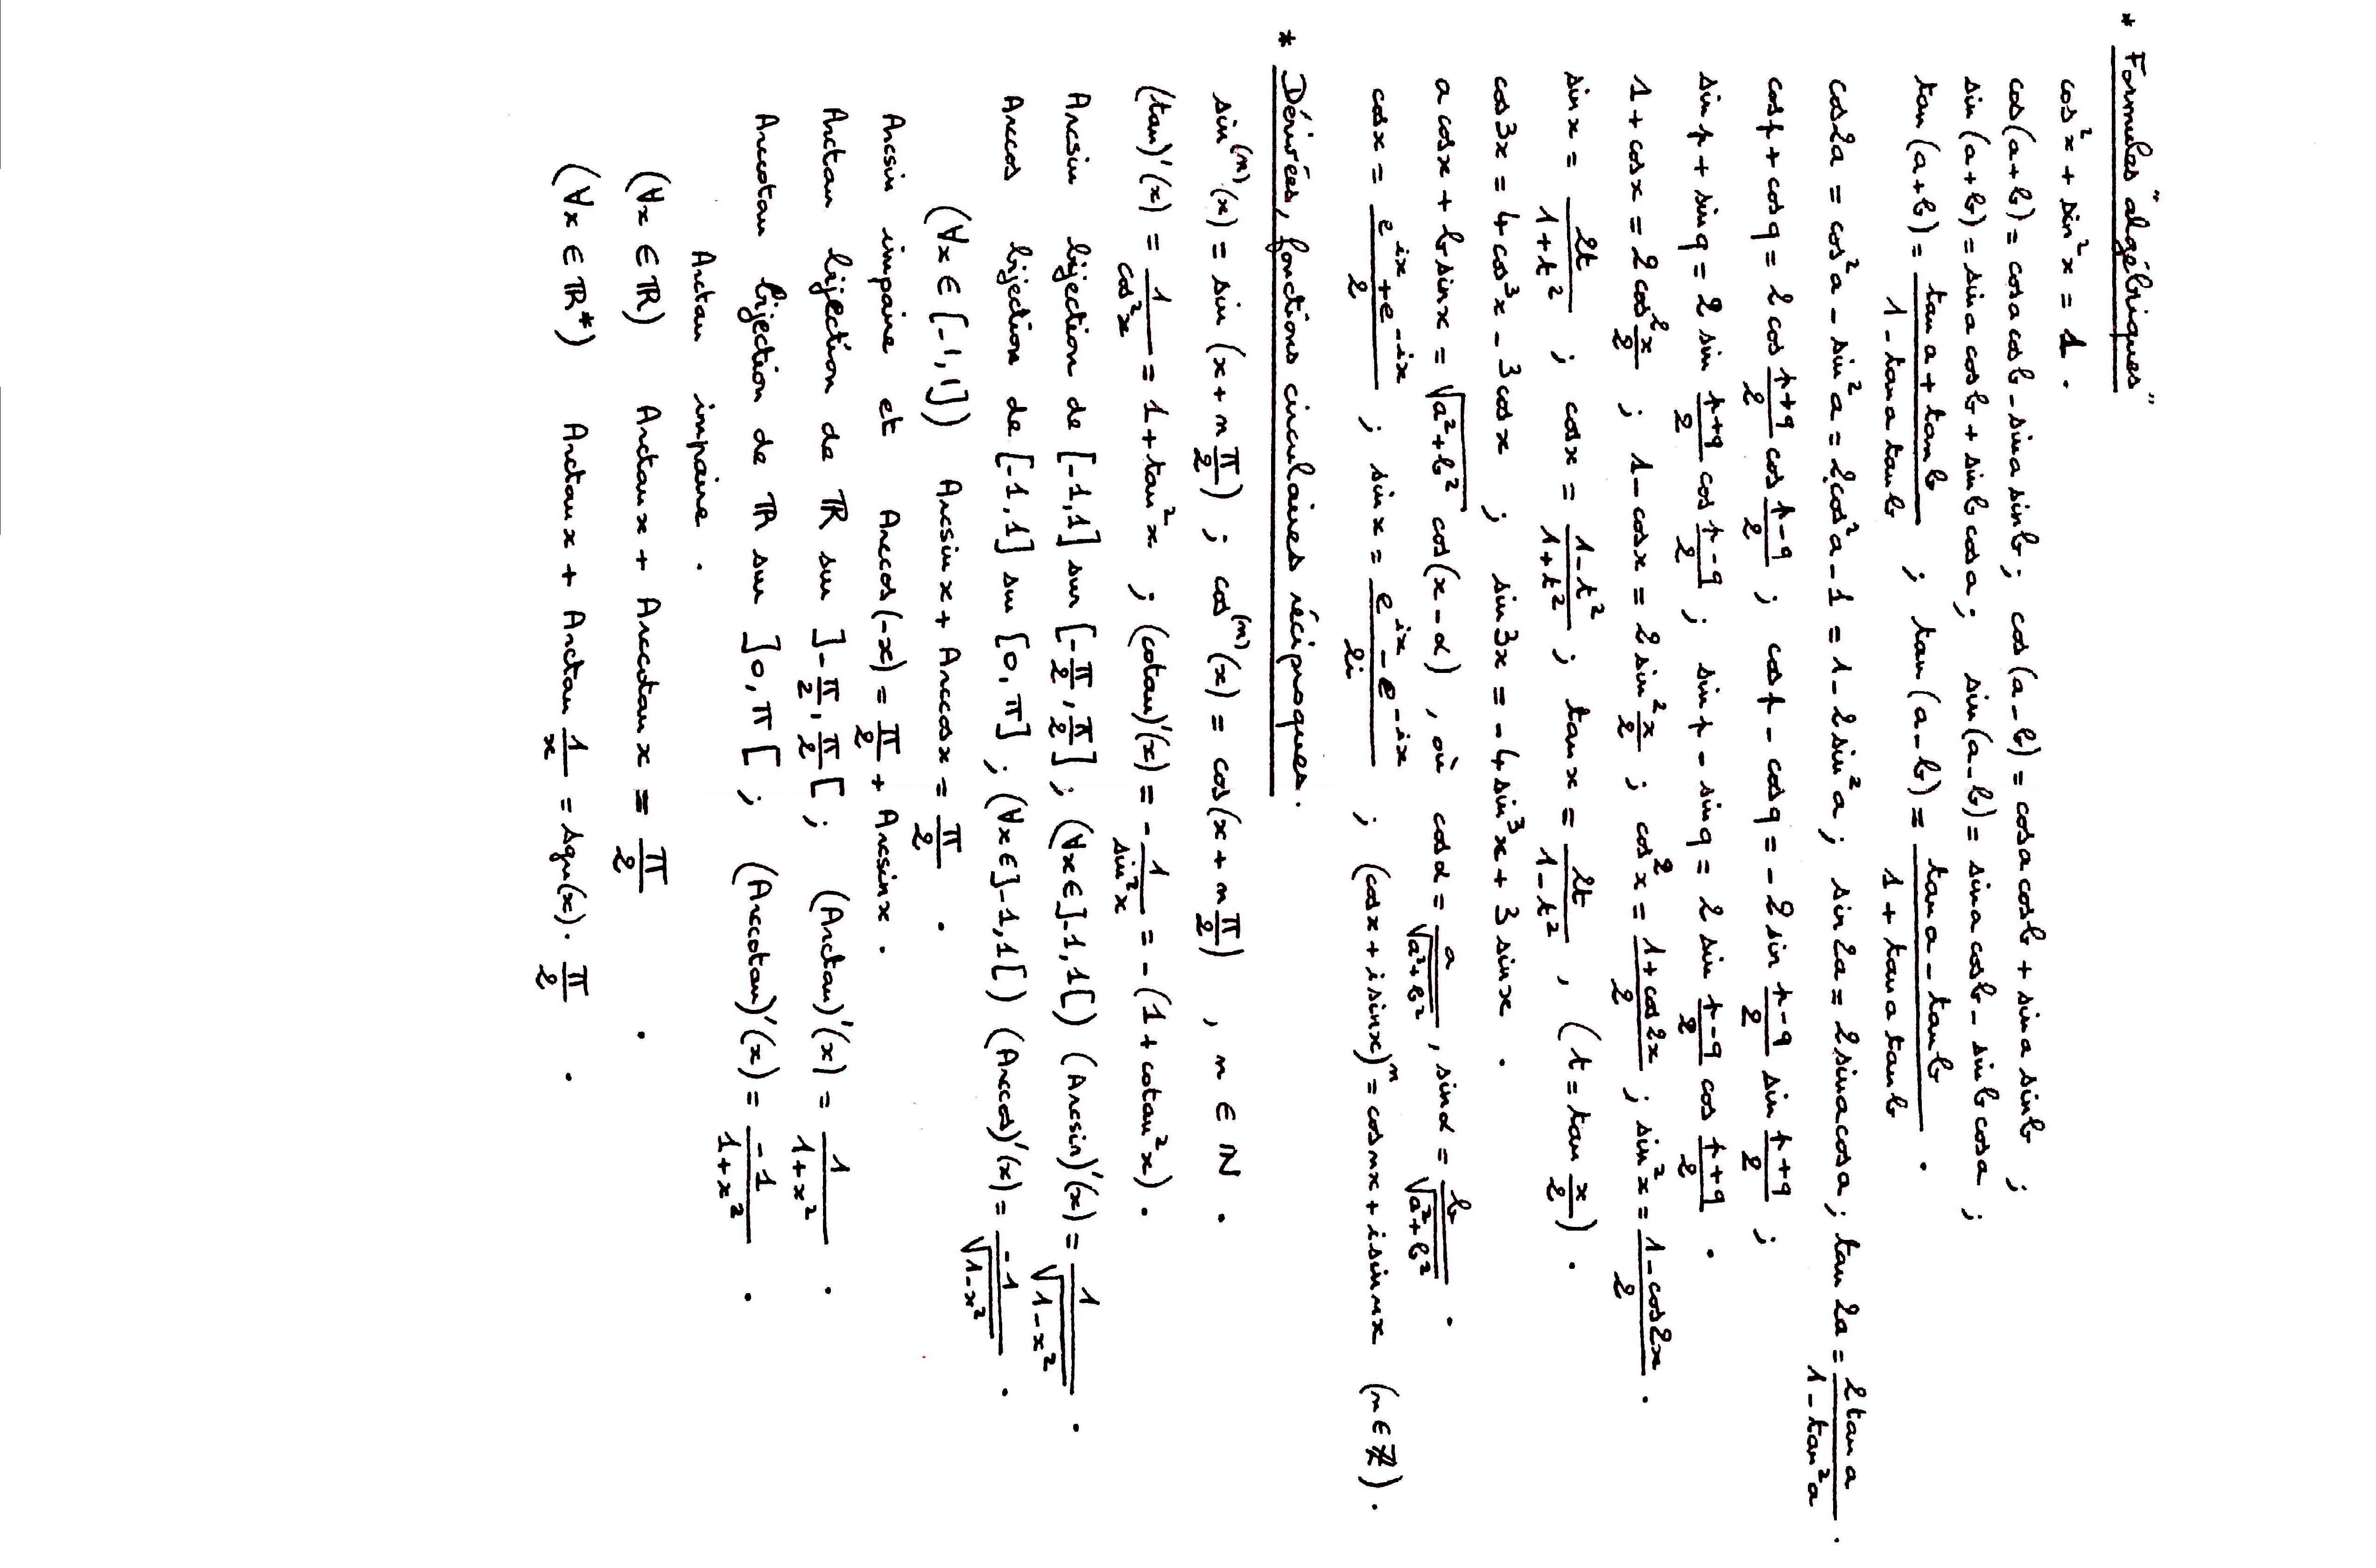
\includegraphics[height=13cm]{trigo}

\end{document}
